\documentclass[10pt]{article}

\usepackage[margin=0.75in]{geometry}
\usepackage{amsmath,amsthm,amssymb}
\usepackage{xcolor}
\usepackage{cancel}
\usepackage{graphicx}
\usepackage{changepage}
\usepackage{circuitikz}
\usepackage{pgfplots}
\usepackage{physics}
\usepackage{hyperref}
\usepackage{minted}
\usepackage[breakable]{tcolorbox}
\usepackage[inline]{enumitem}

\theoremstyle{definition}
\newtheorem{problem}{Problem}
\newtheorem{soln}{Solution}

\pgfplotsset{compat=newest}
\usetikzlibrary{lindenmayersystems}
\usetikzlibrary{arrows}

\definecolor{incolor}{HTML}{303F9F}
\definecolor{outcolor}{HTML}{D84315}
\definecolor{cellborder}{HTML}{CFCFCF}
\definecolor{cellbackground}{HTML}{F7F7F7}
\newcommand{\eq}{=}
\tikzset
{%
  axes/.style={thick,-latex},
  cylinder/.style={right color=blue!80,left color=white,fill opacity=0.7},
  paraboloid back/.style={left color=magenta!80,fill opacity=0.4},
  paraboloid front/.style={left color=white, right color=magenta!80,fill opacity=0.4},
}

\makeatletter
\newcommand{\boxspacing}{\kern\kvtcb@left@rule\kern\kvtcb@boxsep}
\makeatother
\newcommand{\prompt}[4]{
    \ttfamily\llap{{\color{#2}[#3]:\hspace{3pt}#4}}\vspace{-\baselineskip}
}

\newcommand{\highlight}[1]{\colorbox{yellow}{$\displaystyle #1$}}

\newcommand{\volts}[0]{\mathrm{V}}
\newcommand{\amps}[0]{\mathrm{A}}
\newcommand{\ohms}[0]{\Omega}
\newcommand{\farad}[0]{\mathrm{F}}
\newcommand{\coulomb}[0]{\mathrm{C}}
\newcommand{\watts}[0]{\mathrm{W}}

\hypersetup{
    colorlinks=true,
    linkcolor=blue,
    filecolor=magenta,      
    urlcolor=cyan,
    pdftitle={Overleaf Example},
    pdfpagemode=FullScreen,
    }

\NewDocumentCommand{\evalat}{sO{\big}mm}{%
  \IfBooleanTF{#1}
   {\mleft. #3 \mright|_{#4}}
   {#3#2|_{#4}}%
}

\title{Physics 2130: Lab 1}
\author{Jeremy Favro}
\date{\today}

\begin{document}

\maketitle

\begin{minted}[breaklines]{python}
  import matplotlib.pyplot as pyplot
  import numpy as np
  
  # I <3 avoiding code repetition
  def plot_trimmed(path: str, label: str, mintime: float, minpos: float, maxtime: float) -> None:
      data = np.loadtxt(path, delimiter=",", skiprows=1) # does this path syntax work on windows? who knows
      data = data[ # not sure if there's a "smarter" way of doing this
          (data[:, 0] > mintime) & 
          (data[:, 1] > minpos) & 
          (data[:, 0] < maxtime)
      ]
      times = data[:, 0]
      positions = data[:, 1]
      pyplot.plot(times, positions, label=label)
  
  plot_trimmed("./data/run1.csv", "run 1", .45, .1, 2.5)
  
  plot_trimmed("./data/run2.csv", "run 2", .4, .1, 2.2)
  
  plot_trimmed("./data/run3.csv", "run 3", 1, .1, 3)
  
  pyplot.xlabel("Time (s)")
  pyplot.ylabel("Position (m)")
  pyplot.legend()
  pyplot.show()
\end{minted}

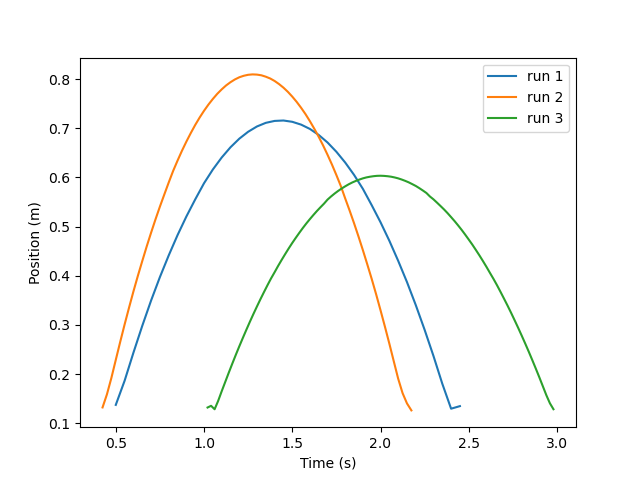
\includegraphics{Figure_1.png}\\
The graph shows the expected motion of an object moving up and then back down a ramp. Each run begins with a steep slope and tapers off to zero before starting
downwards at a shallow slope which becomes steeper with time. This indicates a constant ``downwards'' acceleration due to gravity, which is expected. 
The runs (I believe) differ effectively only in initial velocity with run 3 being the slowest and run 2 the fastest.

\end{document}